% To je predloga za poročila o domačih nalogah pri predmetih, katerih
% nosilec je Blaž Zupan. Seveda lahko tudi dodaš kakšen nov, zanimiv
% in uporaben element, ki ga v tej predlogi (še) ni. Več o LaTeX-u izveš na
% spletu, na primer na http://tobi.oetiker.ch/lshort/lshort.pdf.
%
% To predlogo lahko spremeniš v PDF dokument s pomočjo programa
% pdflatex, ki je del standardne instalacije LaTeX programov.

\documentclass[a4paper,11pt]{article}
\usepackage{a4wide}
\usepackage{fullpage}
\usepackage[utf8x]{inputenc}
\usepackage[slovene]{babel}
\selectlanguage{slovene}
\usepackage[toc,page]{appendix}
\usepackage[pdftex]{graphicx} % za slike
\usepackage{setspace}
\usepackage{color}
\definecolor{light-gray}{gray}{0.95}
\usepackage{listings} % za vključevanje kode
\usepackage{hyperref}
\usepackage{float}
\usepackage{verbatim}
\renewcommand{\baselinestretch}{1.2} % za boljšo berljivost večji razmak
\renewcommand{\appendixpagename}{Priloge}

\lstset{ % nastavitve za izpis kode, sem lahko tudi kaj dodaš/spremeniš
language=Python,
basicstyle=\footnotesize,
basicstyle=\ttfamily\footnotesize\setstretch{1},
backgroundcolor=\color{light-gray},
}

\title{Druga domača naloga}
\author{Anže Pečar (63060257)}
\date{\today}

\begin{document}

\maketitle

\section{Uvod}

Naša naloga je bila izračunati kako informativne so značilke za posamezen razred. Podatke smo najprej binarilizirali in nato izračunali medsebojno informacijo. Na koncu smo s pomočjo permutacijskega testa določili kateri atributi so značilni za posamezen razred. Delali smo na zmanjšanem naboru podatkov, ki jih uporablja tekmovanje \textit{JRS 2012 Data Mining Competition: Topical Classification of Biomedical Research Papers}.

\section{Metode}
\subsection{Količina medsebojne informacije}
Na predavanjih smo količino medsebojne informacije definirali kot

\[ 
	I(X;Y) = H(Y) - H(Y|X)
\]
pove pa nam koliko informacije prispeva posamezen atribut. $H$ predstavlja entropijo, ki je definirana kot:
\[
	H(A) = p * log_2 {1 \over p}
\]
Za primer bomo izračunali medsebojno informacijo za razred $c40$ in atribut $D_0$. Razred $c40$ ima $1498$ vrednosti $F$ in $502$ vrednosti $T$, kar pomeni, da je njegova entropija enaka 
\[
	H(c40) = H({1498 \over 2000}, {502\over 2000}) = 0.812859243
\]
Za atribut $D_0$ pa je razporejen po naslednji tabeli:

\begin{tabular}{r|l}
  1489 & $D_0=0$ in $c40=F$ \\
  501 & $D_0=0$ in $c40=T$ \\
  9 & $D_0 = 1$ in $c40=F$ \\
  1 & $D_0 = 1$ in $c40=T$ \\
\end{tabular}

S pomočjo zgornje tabele lahko izračunamo $H(c40|D_0)$:

\[
	H(c40|D_0) = {10\over2000}*H({9\over2000}, {1\over2000}) + {1990\over2000}*H({1489\over2000}, {501\over2000}) = 0.812322554
\]
Količino medsebojne enakosti dobimo tako, da dobljeni vrednosti odštejemo:
\[
	I(D_0;c40) = H(c40) - H(c40|D_0) = 0.000536689
\]
Če nad istimi podatki poženemo še funkcijo InformationGain iz paketa Orange dobimo podoben rezultat:
\[
I(D_0;c40) = 0.0005311369895935059
\]

Izračun količine medsebojne informacije nam sam po sebi še ne pove ali je atribut povezan z razredom. Zato uporabimo tako imenovani \textbf{permutacijski test}, ki poteka tako, da naredimo določeno število naključnih permutacij vrednosti razreda. Za te naključne permutacije izračunamo InformationGain. Če je odstotek tako dobljenih vrednosti večji od vrednosti $Alphe$ našo hipotezo, da je atribut povezan z razredom, lahko zavrnemo. Če pa je odstotek tako dobljenih vrednosti manjši $Alphe$ pa lahko zavrnemo obratno hipotezo, da atribut in razred nista povezana. 
\section{Rezultati}
\subsection{Grafi}

Delovanje svojega algoritma sem najprej preizkusil nad alpha vrednostjo 0.0. Rezultati so vidni na Slikah \ref{skupno100} in \ref{skupno100a} - prvi graf. Zanimalo me je tudi, kako vpliva velikost alphe na informativnost značilk. Algoritem sem zato pognal za alpho vrednost 0.01 in 0.05. Rezultati so na Slikah \ref{skupno100} in \ref{skupno100a} drugi in tretji graf.

\begin{figure}[H]
\begin{center}
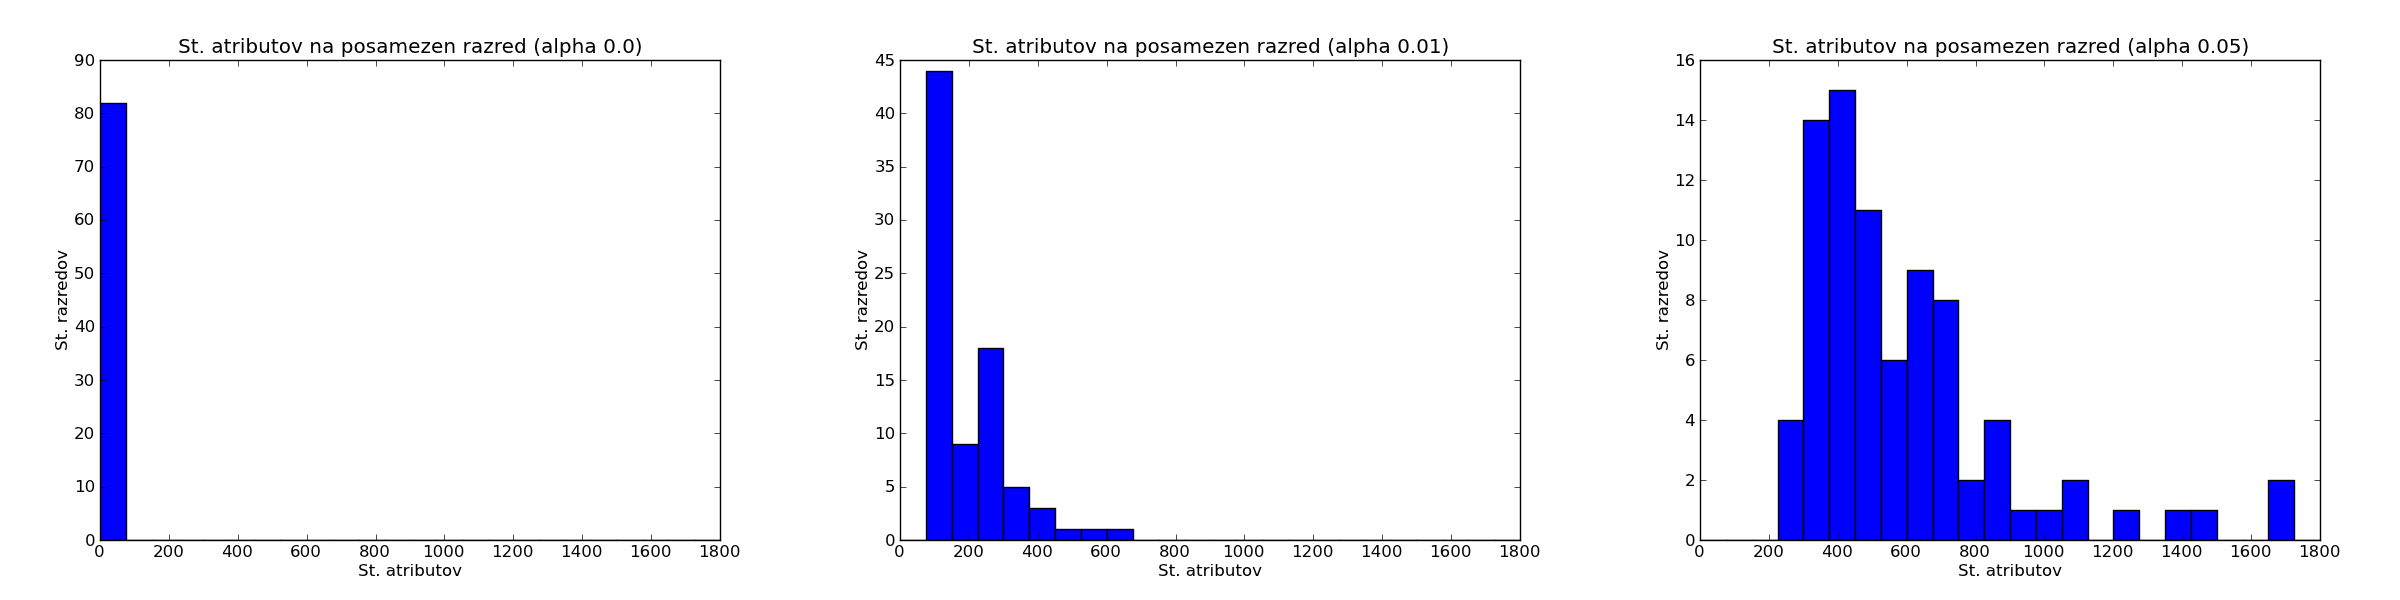
\includegraphics[scale=0.2]{skupno100.png}
\caption{Rezultati 100 permutacij za različne vrednosti Alpha}
\label{skupno100}
\end{center}
\end{figure}
Slika \ref{skupno100} prikazuje število atributov na posamezen razred za različne vrednosti alpha (0.0, 0.01 in 0.05).   
\begin{figure}[H]
\begin{center}
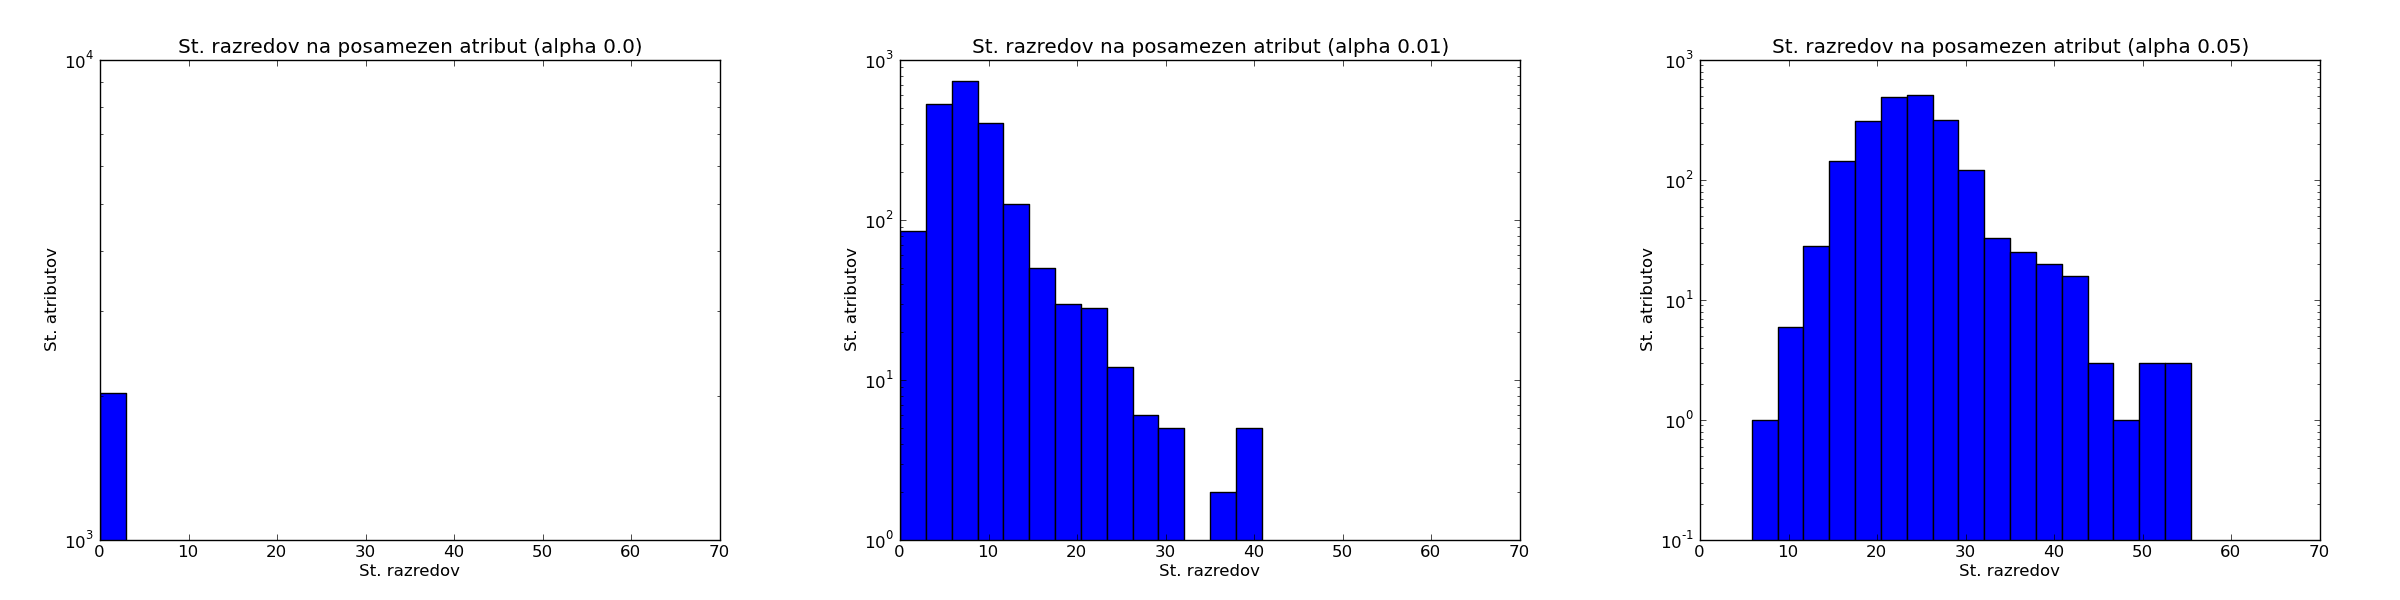
\includegraphics[scale=0.2]{skuptnoAttr100-log.png}
\caption{Rezultati 100 permutacij za različne vrednosti Alpha, logaritemska skala}
\label{skupno100a}
\end{center}
\end{figure}

Slika \ref{skupno100a} pa prikazuje št. razredov na posamezen atribut. Za lepši prikaz sem uporabil logaritemsko skalo.

\begin{figure}[H]
\begin{center}
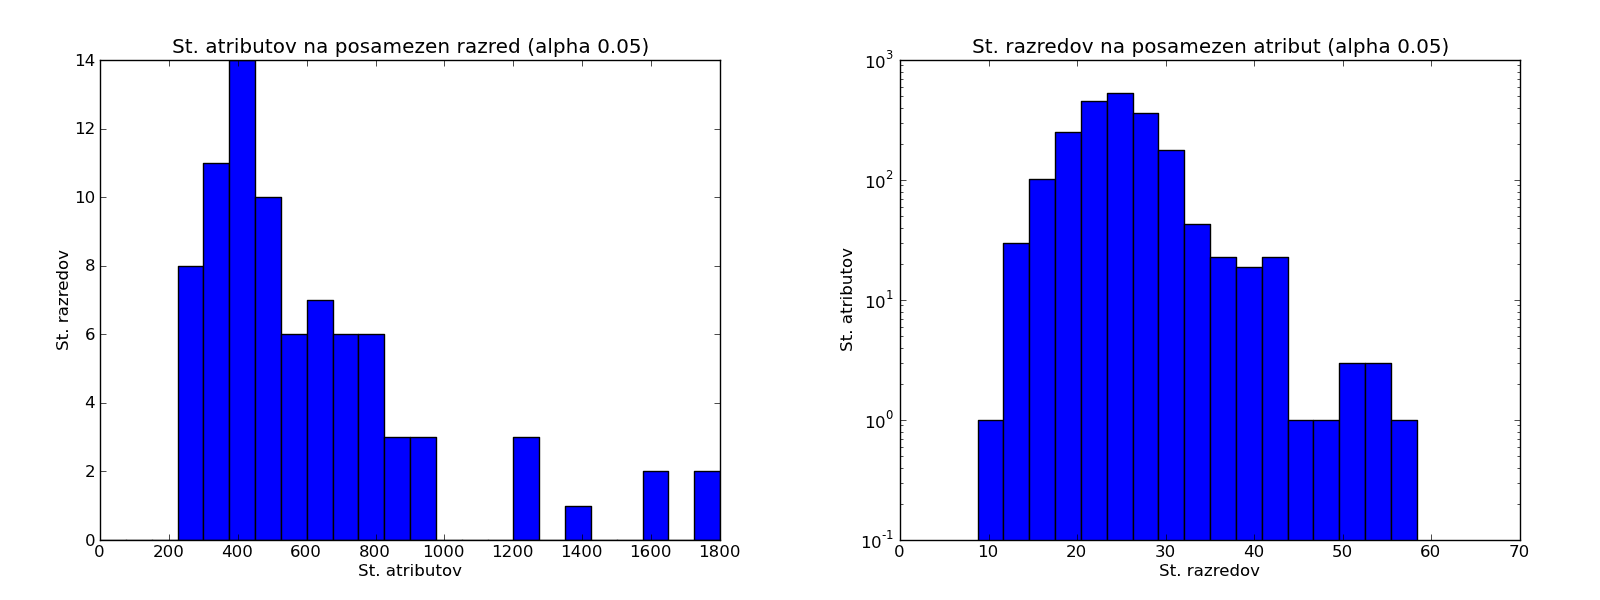
\includegraphics[scale=0.2]{skupno500.png}
\caption{Rezultati 500 permutacij}
\label{skupno500}
\end{center}
\end{figure}

Na koncu sem pognal moj algoritem še za 500 permutacij, tokrat za alpho vrednost 0.05. Rezultata sta vidna na Sliki \ref{skupno500}.


\subsection{Hitrost izvajanja}
10 permutacij:
\begin{verbatim}
real	8m20.437s
user	8m18.875s
sys	0m0.628s
\end{verbatim}
100 permutacij:
\begin{verbatim}
real	73m46.716s
user	73m36.088s
sys	0m2.380s

\end{verbatim}
500 permutacij:
\begin{verbatim}
real	377m52.873s
user	377m18.379s
sys	0m7.308s
\end{verbatim}

Čas izvajanja sem želel pohitriti z boljšo izrabo dveh jeder mojega prenosnika. Za ta namen sem najprej napisal verzijo programa z nitmi. Uporabil sem funkcijo map iz razreda Pool, ki razdeli izvajanje funkcije v posamezne niti. Št. niti je določeno v konstruktorju. Ker pohitritve v delovanju nisem opazil, sem sklepal, da je problem, ker sta obe niti dostopali do seznama, kjer so se shranjevali rezultati.

Ker rešitev z nitmi ni delovala zadovoljivo, sem se odločil poskusiti še z dvema ločenima procesoma. Program sem spremenil tako, da je prvi proces računal vrednosti za lihe razrede, drugi pa za sode, vendar tudi tukaj nisem opazil nobene pohitritve. Še več, oba procesa s polovičnim naborom razredov sta se izvajala dalj časa, kot pa en proces s polnim naborom razredov. Skelpam, da je to posledica velike količine dostopov do RAMa, in malo starejše arhitekture procesorja (Core 2 Duo). Na Core iX procesorjih s HyperThreading tehnologijo bi morala dvoprocesna verzija programa delovati bolje. 

\section{Izjava o izdelavi domače naloge}
Domačo nalogo in pripadajoče programe sem izdelal sam.
\end{document}
